\documentclass[oneside,a4paper,12pt]{book}
\usepackage{fancyhdr}

\fancypagestyle{plain}{%
  \fancyhf{}
  \fancyfoot[CE]{Pune Institute of Computer Technology, Department of Computer Engineering 2018 19}
  \fancyfoot[RE]{\thepage}
}
\pagestyle{fancy}
\fancyhead{}
\renewcommand{\headrulewidth}{0pt}
\footskip = 0.625in
\cfoot{}
\rfoot{}

\usepackage[]{hyperref}
\usepackage{tikz}
\usetikzlibrary{arrows,shapes,snakes,automata,backgrounds,petri}
\usepackage{titlesec}
\usepackage{tabularx}

\usepackage[nottoc,notlot,notlof,numbib]{tocbibind}
\usepackage[titletoc]{appendix}
\usepackage{titletoc}
\renewcommand{\appendixname}{Annexure}
\renewcommand{\bibname}{References}

\setcounter{secnumdepth}{5}

\usepackage{float}
\usepackage{subcaption}
\usepackage{multirow}
\usepackage{lmodern}

\usepackage{algorithm}
\usepackage{algorithm2e}
\usepackage{algorithmic}
\usepackage{amsmath}
\usepackage[utf8]{inputenc}
\usepackage{mathtools}
\usepackage{tabu}
\newcommand\Myperm[2][^n]{\prescript{#1\mkern-2.5mu}{}P_{#2}}
\newcommand*\xor{\mathbin{\oplus}}

\usepackage[utf8]{inputenc}
 
\usepackage{nomencl}
\makenomenclature
\usepackage{array}
\usepackage[utf8]{inputenc}
\usepackage{graphicx}
\usepackage{tabularx}

\begin{document}

\setlength{\parindent}{0mm}
\begin{center}
{\bfseries A PROJECT REPORT ON \\}
 \vspace*{2\baselineskip}
{\bfseries \fontsize{16}{15} \selectfont CODE IMPACT ANALYZER \\ \vspace*{2\baselineskip}}
{\fontsize{12}{12} \selectfont SUBMITTED TO THE SAVITRIBAI PHULE UNIVERSITY, PUNE
 \\ IN THE PARTIAL FULFILLMENT OF THE REQUIREMENTS \\ FOR THE AWARD OF THE DEGREE  \\
 \vspace*{1\baselineskip}
 OF

\vspace*{2\baselineskip}}
{\bfseries \fontsize{16}{12} \selectfont\mbox{BACHELOR OF ENGINEERING}\\ \vspace{2mm}{\bfseries \fontsize{16}{12} \selectfont\mbox{(COMPUTER ENGINEERING)} \\
\vspace*{2\baselineskip}} 
{\bfseries \fontsize{12}{12} \selectfont SUBMITTED BY \\ 
\vspace*{2\baselineskip}} 
{\bfseries \fontsize{12}{12} \selectfont
\begin{center}
\begin{tabular}{ l c c }
 AMEYA BABHULGAONKAR &  & Exam No: B150054217 \\ 
\quad PRASHANT BHIVSANE&  & Exam No: B150054233\\  
\quad \quad CHAITNYA JOSHI &  & Exam No: B150054314\\
\quad \quad \quad ROHIT DOSHI &  & Exam No: B150054266\\
 

\end{tabular}
\end{center}

\vspace*{1\baselineskip}}


\includegraphics[width=100pt]{collegelogo.png} \\
\vskip 0.5cm
{\bfseries \fontsize{16}{15} \selectfont
{\bfseries \fontsize{12}{12} \selectfont 
DEPARTMENT OF COMPUTER ENGINEERING\\
\vspace*{1\baselineskip}
PUNE INSTITUTE OF COMPUTER TECHNOLOGY \\
\vspace*{1\baselineskip}
DHANKAWADI, PUNE - 411043

\vspace*{1\baselineskip}
SAVITRIBAI PHULE PUNE UNIVERSITY\\
2018-2019
\vspace*{1\baselineskip}

\end{center}

\newpage

{\bfseries \fontsize{12}{12} \selectfont }

\begin{figure}[ht]
\centering

\includegraphics[width=100pt]{collegelogo.png}
\end{figure}

{\bfseries \fontsize{14}{12} \selectfont \centerline{CERTIFICATE} 
\vspace*{2\baselineskip}}

\centerline{This is to certify that the project report entitled}
\vspace*{1\baselineskip} 


{\bfseries \fontsize{12}{12} \selectfont 
\begin{center}
    {``CODE IMPACT ANALYZER''}
\end{center}}
{\bfseries \fontsize{12}{12} \selectfont \centerline{  }
\vspace*{1\baselineskip}}

\centerline{Submitted by}
\vspace*{1\baselineskip} 

{\bfseries \fontsize{12}{12} \selectfont
\begin{center}
\begin{tabular}{ l c c }
 AMEYA BABHULGAONKAR &  & Exam No: B150054217 \\ 
\quad PRASHANT BHIVSANE&  & Exam No: B150054233\\  
\quad \quad CHAITNYA JOSHI &  & Exam No: B150054314\\
\quad \quad \quad ROHIT DOSHI &  & Exam No: B150054266\\
\end{tabular}
\end{center}

\vspace*{1\baselineskip}}

is a bonafide student of this institute and the work has been carried out by him/her under the supervision of \textbf{Prof. K. C. Waghmare} and it is approved for the partial fulfilment of the requirement of Savitribai Phule Pune University, for the award of the degree of \textbf{Bachelor of Engineering} (Computer Engineering). \\
\\
\vskip 1cm
\bgroup
\def\arraystretch{0.7}
\begin{tabular}{c c }
\textbf{Prof. K. C. Waghmare} &  \hspace{50 mm} \textbf{Dr. R. B. Ingle} \\
Internal Guide,   &  \hspace{50 mm} Head, \\
Dept. of Computer Engg.  &	\hspace{50 mm}Dept. of Computer Engg. \\
\end{tabular}

\begin{center} 
\vspace*{1\baselineskip}
{
\textbf{Dr. P. T. Kulkarni}\\
Principal,\\
Pune Institute of Computer Technology  
}
\end{center}

Place: Pune\\
Date:

{\newpage {\bfseries \fontsize{14}{12} \selectfont \centerline{ACKNOWLEDGEMENT} 
\vspace*{2\baselineskip}} \setlength{\parindent}{11mm} }
{\setlength{\parindent}{0mm} }

\begin{justify}

It gives us great pleasure in presenting the project report on ‘Code Impact Analyzer’. We would like to take this opportunity to thank our internal guide Prof. K. C. Waghmare for giving us all the help and guidance we needed. We are really grateful to them for their kind support. Their valuable suggestions were very helpful.
\end{justify}\par
\begin{justify}

We are also grateful to Prof. Dr. Rajesh B. Ingle, Head of Computer Engineering Department, PICT for his indispensable support, suggestions.
\end{justify}\par
\begin{justify}

In the end our special thanks to Mr. Manish Kotulkar and Mr. Ranjit Jadhav, BMC Software, Pune for providing various resources with all needed software platforms, for our project.
\end{justify}\par

\vspace*{2\baselineskip} 

\begin{tabular}{p{8.70cm}r}
&Ameya Babhulgaokar\\[3pt]
&Prashant Bhivsane \quad   \\[3pt]
&Chaitnya Joshi \quad \quad \\[3pt]
&Rohit Doshi \quad \quad \quad \\
&(B. E. Computer Engineering)
\end{tabular}

{\newpage {\bfseries \fontsize{14}{12} \selectfont \centerline{ABSTRACT} 
\vspace*{2\baselineskip}} 
\setlength{\parindent}{11mm} }
{\setlength{\parindent}{0mm} }
\begin{justify}
Defect prediction is currently the area of an undergoing research.  But instead of predicting defects focus of researchers has now been changed to predicting risky software changes(patches) which would create or open more defects in other files.
\end{justify}\par
\begin{justify}
We have used historical project data which will include changes made to any project’s files and the number of issues caused by those changes.   We have prepared our own dataset using this data and have classified the files into risky, non-risky and neutral classes.
\end{justify}\par
\begin{justify}
Source Code Control systems(eg.git,svn) and defect tracking systems(eg.JIRA) will together provide the historical data required for the project.
\end{justify}\par

\vspace*{1\baselineskip}
\vspace*{1.5\baselineskip}

\tableofcontents

\pagenumbering{roman}
\addcontentsline{toc}{section}{List of Abbreviations} \newpage
\addcontentsline{toc}{section}{List of Figures} \newpage
\addcontentsline{toc}{section}{List of Tables}

\newpage 
%list of abbreviations


\vspace{\baselineskip}

\vspace{\baselineskip}

\vspace{\baselineskip}

\vspace*{4\baselineskip}

{\fontsize{24pt}{30pt}\selectfont \textbf{List of Abbreviations}\par}\par


\vspace*{3\baselineskip}
\textbf{API}\ \ \ \ \ \   Application Program Interface\par

\textbf{REST\ \ \  }Representational State Transfer\par

\textbf{SDLC  \  }  Software Development Life Cycle\par

\textbf{ANN\ \ \ } Artificial Neural Network\par

\textbf{IDE\ \ \ \ \ } Integrated Development Environment\par

\textbf{HTML\ } Hypertext Markup Language\par

\textbf{UML\ \  \ } Unified Modeling Language\par

\textbf{HTTP\ \  \ }HyperText Transfer Protocol\par

\textbf{RAM\ \  \ \ }Random Access Memory\par

\textbf{PDE\ \  \ \ \ }Plugin Development Environment\par

\textbf{JAR\ \  \ \ \ }Java Archive\par

\textbf{CPU\ \  \ \ }Central Processing Unit\par

\vspace{\baselineskip}

\vspace{\baselineskip}

\newpage








\listoffigures 
\listoftables


\mainmatter

\titleformat{\chapter}[display]
{\fontsize{16}{15}\filcenter}
{\vspace*{\fill}
 \bfseries\LARGE\MakeUppercase{\chaptertitlename}~\thechapter}
{1pc}
{\bfseries\LARGE\MakeUppercase}
[\thispagestyle{empty}\vspace*{\fill}\newpage]

\setlength{\parindent}{11mm}
\rfoot{Page \thepage}

\pagestyle{fancy}
\fancyhf{}
\lhead{Code Impact Analyzer}
\cfoot{PICT, Department of Computer Engineering 2018-19}
\rfoot{Page \thepage}
\renewcommand{\headrulewidth}{2pt}
\renewcommand{\footrulewidth}{1pt}

\chapter{Introduction}

\section{Overview}
\setlength{\parskip}{0.0pt}
	\item A main objective of this project is to provide a system for reviewing files during the development phase. Reviewing includes checking severity of a file and provide few of the other details associated with it which will help developers to know about the past statistics of queried file.\par

\setlength{\parskip}{9.96pt}
	\item This system will predict the severity class for a given file(low, medium, high) and based on that, the developer might know about what could be the cost of dealing with the given file and what are the major problem areas that are occurred to be problematic which might open defects in near future.\par

\section{Motivation}
\setlength{\parskip}{0.0pt}
\begin{itemize}
	\item Open source has brought the concept of distributed development of application.\par

	\item The Version Control Systems(VCS) play crucial role in development of such systems. Also Defect Tracking Tool like JIRA are majorly used.\par

	\item After pushing code for review, the developer might have no idea if he/she is going to see his work reflected in the final product. Also, even code reviewer cannot talk about efficiency of code snippet and how much error it can open in the overall development.
\end{itemize}\par

\setlength{\parskip}{9.96pt}
\pagebreak \par

\section{Problem Definition and Objectives}
\begin{justify}
Given\ a project, its specific package and a file in that project, we will able to predict the impact of software change  made in that file. We will predict the impact of a software change(s) using the file history associated with Git and JIRA.
\end{justify}\par

\section{Project Scope \& Limitations }
\setlength{\parskip}{0.0pt}
\begin{itemize}
	\item Plugin will receive file name as a input from user and it will return severity of the given file as a output to user on a webpage.\par

\setlength{\parskip}{9.96pt}
	\item It is easy to use tool which uses ANN model deployed over server to return severity class to developer. Developer instead of going to Git and checking JIRA, and analyzing file details manually can directly get file details at few clicks.\par
	
	\item Plugin requires a file to be present in the database.\par
\end{itemize}

\section{Methodologies of problem solving and efficiency issues}
\setlength{\parskip}{0.0pt}
\begin{itemize}
    \item
     A research was done over a dataset to determine which of all the features are actually turning out to be significant for determining the severity of given file. Thus only the required features were used for training a model.
    \par
    \item
    As the data gathered from Git and JIRA is not labelled, it has been clustered as labeled data is fed into an ANN model. K-means gave back clusters as 'Low', 'Medium', 'High'.
    \par
    	\item Artificial Neural Network model is used  for multi-class classification of obtained dataset into Low, Medium and High severity.\par
\end{itemize}


\section{Outcome}
\setlength{\parskip}{0.0pt}
\begin{itemize}
    \item An Eclipse plugin is developed, so that developers can use it.\par
\end{itemize}
	

\chapter{Literature Survey}


\section{Literature Survey}


\subsection{Continuous Defect Prediction: The Idea and a Related Dataset[1]}

\setlength{\parskip}{0.0pt}
\textbf{Keywords:}\par

\textbf{ }Mining\ software repositories, defect prediction, continuous defect prediction,  software repository, open science\\
\setlength{\parskip}{0.0pt}
\textbf{Abstract:}\par

\begin{justify}
\textbf{ }
In this paper[1], authors have shared the dataset which can be used for continuous defect prediction.They have used GitHub as source code control system and they have used LibGit2Sharp library.Their dataset embraces 1265 software projects, 30,022 distinct commit authors and several software process metrics that in earlier research appeared to be useful in software defect prediction.Their process metrics include various factors such as Number Of Revisions,Number Of Distinct Committers,Number Of Modified Lines etc. 
\end{justify}\par



\subsection{Prediction of Defect Susceptibility in Object Oriented Software[2]}

\setlength{\parskip}{0.0pt}
\textbf{Keywords}: \par

Object oriented, software metrics, cohesion, coupling, defect proneness, fault prediction, defect propagation factor\\
\setlength{\parskip}{0.0pt}
\textbf{Abstract:}\par

\begin{justify}
\textbf{ }
In\ this\ project[2],  they have tried to identify the defect prone software portions.They have implemented this system for Object Oriented System and that too for projects developed in java.For each class they calculated the 7 different metrics using which they predict defect prone software portions.Different metrics include  number of methods in a class ,depth of inheritance tree ,numbers of children ,coupling between objects,Afferent coupling,Lack of cohesion in methods and cohesion among methods.Using the calculated defect propagation factor they are predicting defect prone software portions.\par 
\end{justify}\par
\newpage

\subsection{Defect Association and Complexity Prediction by Mining Association and Clustering Rules[3]}

\setlength{\parskip}{0.0pt}
\textbf{Keywords}: \par

Defect Associations, Clustering, Defect Correction Effort, Defect association\\
\setlength{\parskip}{0.0pt}
\textbf{Abstract:}\par

\begin{justify}
\textbf{ }
Software defect prediction is combined with association rule mining to determine the associations that occur among the detected defects and the effort required for isolating and correcting these defects. They have used clustering techniques to classify the defects into three classes viz. Simple,Moderate and complex. They have also predicted the defect correction efforts using metrics such as defect type,typological error,bad code and omission error.Based on weighted analysis method, it is determined whether the presence of a particular defect might affect the project schedule significantly.\par
\end{justify}\par


\subsection{Connecting Software Metrics across Versions to Predict Defects[4]}

\setlength{\parskip}{0.0pt}
\textbf{Keywords:}\par

Defect Prediction,Recurrent Neural Networks(RNN).\\
\setlength{\parskip}{0.0pt}
\textbf{Abstract:}\par

\begin{justify}
\textbf{ }
They[4]\ have\ \ proposed  the  use of the Historical Version Sequence of Metrics (HVSM) in continuous software versions as defect predictors\textbf{.}They\ have used Recurrent Neural Network to take HVSM as input to build prediction models.They have focused  on improving the performance in Within Project Defect Prediction(WPDP) with their approaches. HVSM can reveal the files’ comprehensive change history which are not included in most process metrics.\par
\end{justify}\par
\newpage
\section{Literature Survey Table}


\begingroup
\setlength{\tabcolsep}{10pt} % Default value: 6pt
\renewcommand{\arraystretch}{1.5} % Default value: 1

\begin{table}[H]
 			\centering
\begin{tabular}{p{1.77in}p{1.95in}p{1.95in}}
\hline
%row no:1
\multicolumn{1}{|p{1.77in}}{Paper Name} & 
\multicolumn{1}{|p{1.95in}}{Tool/Algorithms used} & 
\multicolumn{1}{|p{1.95in}|}{Conclusion} \\ 
\hline
%row no:2
\multicolumn{1}{|p{1.77in}}{Continuous Defect Prediction: The Idea and a Related Dataset[1] \par } & 
\multicolumn{1}{|p{1.95in}}{Github, LibGit2Sharp library} & 
\multicolumn{1}{|p{1.95in}|}{Dataset from both open source and commercial projects is used . } \\
\hline
%row no:3
\multicolumn{1}{|p{1.77in}}{Prediction of Defect Susceptibility in Object Oriented Software[2]} & 
\multicolumn{1}{|p{1.95in}}{Neural Network Classifiers} & 
\multicolumn{1}{|p{1.95in}|}{Class which is less cohesive is coupled with another class, then there exists a chance for fault proneness among them.} \\
\hline
%row no:4
\multicolumn{1}{|p{1.77in}}{Defect association and complexity prediction by mining association and clustering rules.[3]} & 
\multicolumn{1}{|p{1.95in}}{Clustering,Association rule mining} & 
\multicolumn{1}{|p{1.95in}|}{Defects are classified and used to predict their impact on software product. } \\
\hline
%row no:5
\multicolumn{1}{|p{1.77in}}{Connecting Software Metrics across Versions to Predict Defects[4]} & 
\multicolumn{1}{|p{1.95in}}{Source code metrics across different versions are used in defect predictors} & 
\multicolumn{1}{|p{1.95in}|}{Source code metrics change across the versions and help in effectively predicting defects.} \\
\hline}

\end{tabular}\caption{Literature Survey Table}
\label{tab:Literature Survey Table}

 \end{table}
 \endgroup



\chapter{Software Requirements Specification}

\section{Introduction}
\subsection{Project Scope}
\setlength{\parskip}{0.0pt}
\begin{itemize}
	\item The project will be effectively used in Software Development Process.\par

	\item It will help Code Reviewer and Tester to ease the defect tracking process.\par
	
	\item It will save time for both Code Reviewer and Software Testers by making the process less manual.


\end{itemize}\par

\subsection{User Classes and Characteristics}
\begin{itemize}

    \item Developer: A person responsible writing code to develop a software.\par

	\item Code Reviewer: A person reviewing code and filing defects.\par

	\item Tester: A person responsible for performing various testing activities.
\end{itemize}\par
    


\section {Functional Requirements}
\subsection{Database Component Agent}
\setlength{\parskip}{0.0pt}
\begin{itemize}
	\item Agent collects and stores defect data.\par

	\item Agent works primarily with JIRA and Git.\par

	\item Agent stores information about defect in database.
\end{itemize}\par

\subsection{Server Component Agent}

\setlength{\parskip}{0.0pt}
\begin{itemize}
	\item Agent uses REST API for communication.\par

	\item Agent facilitates User.\par

	\item Uses Artificial Neural Network.
\end{itemize}\par

\subsection{Client Component Agent}
\begin{itemize}
	\item An Eclipse plugin.\par

	\item Interacts with server and gives back file severity.
\end{itemize}\par

\newpage
\section{Non Functional Requirements}

\begin{justify}
The non-functional requirements of the system include :
\end{justify}\par

\setlength{\parskip}{0.0pt}
\begin{itemize}
	\item System should have suitable user interface.\par

	\item It should be able to detect wrong input given to the system.\par

	\item System should be reliable. Reviewers and developers should be able to see same kind of data when enquired about a file.\par


	\item System should be generic in nature. It should be able to work across different kinds of source control and defect tracking tools.
\end{itemize}\par





\section{External Interface Requirements}

\subsection{User Interfaces}
\begin{itemize}
    \item User Interface is exposed to end user(developer) is through Eclipse plugin.\par
    \item The prediction page is shown up in a browser window.
\end{itemize}

\section{System Requirements}
\subsection{Software Requirements}
\setlength{\parskip}{0.0pt}
\begin{itemize}
	\item Git.\par

	\item JIRA.\par

	\item Python 3.7\par

	\item PyCharm.\par

	\item Java.\par

	\item Eclipse IDE.\par

	\item PostGREs database.\par

	\item Flask\  Server.
	\item MobaXterm\par
	\item WinScp \par
\end{itemize}\par


\subsection{Hardware Requirements}

\setlength{\parskip}{0.0pt}
\begin{itemize}
	\item 32/64 bit Machine\par

	\item 4GB RAM\par

\setlength{\parskip}{9.96pt}
	\item Server with good configuration having 8GB RAM(min) and GPU.
\end{itemize}\par




\section{Analysis Model}

\begin{justify}
Waterfall model :
\end{justify}\par

\setlength{\parskip}{0.0pt}
\begin{itemize}
	\item The waterfall model is a relatively linear sequential design approach for certain areas of engineering design. In software development, it tends to be among the less iterative and flexible approaches.\par

	\item Clearly defined stages.\par

	\item Requirements are very well documented, clear and fixed.\par

	\item There are no ambiguous requirements.\par

	\item Easy to manage due to the rigidity of the model. Each phase has specific deliverables and a review process.\par
\end{itemize}
\section{System Implementation}
\setlength{\parskip}{0.0pt}
\begin{itemize}

	\item Collect defect data from JIRA-Git Integration\par

	\item Develop Server Application\par

	\item Prepare database schema.\par

	\item Develop Client Application ( Eclipse plugin)\par

	\item Deploy Application
\end{itemize}\par

\newpage
\chapter{System Design}

\section{System Architecture}

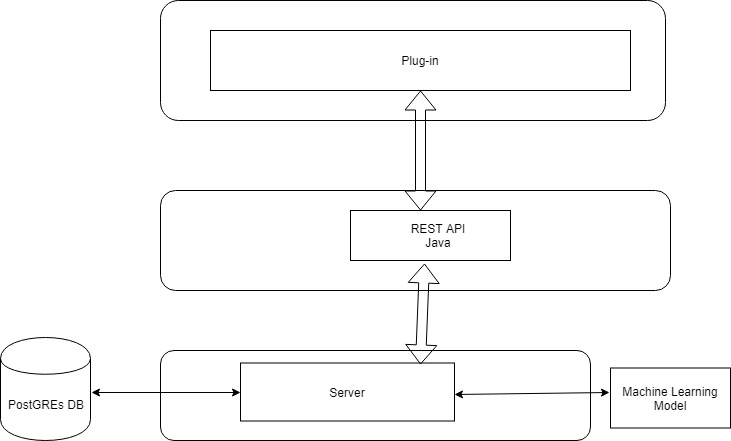
\includegraphics[width=\textwidth]{archi.jpg}
\begin{figure}[h]
    \caption{Architecture Diagram}
    \label{fig:Architecture of Code Impact Analyzer}
\end{figure}

\section{UML Diagrams}

\subsection{Sequence Diagram}
\vspace*{1\baselineskip}
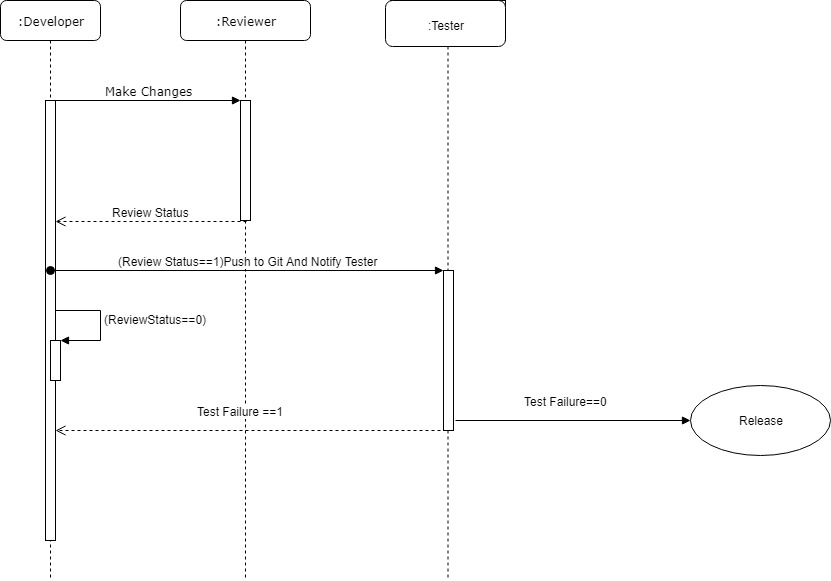
\includegraphics[width=\textwidth]{sequence.png}
\begin{figure}[h]
    \caption{Sequence Diagram}
    \label{fig:Sequence Diagram}
\end{figure}

\subsection{Use Case Diagram}
\vspace*{1\baselineskip}
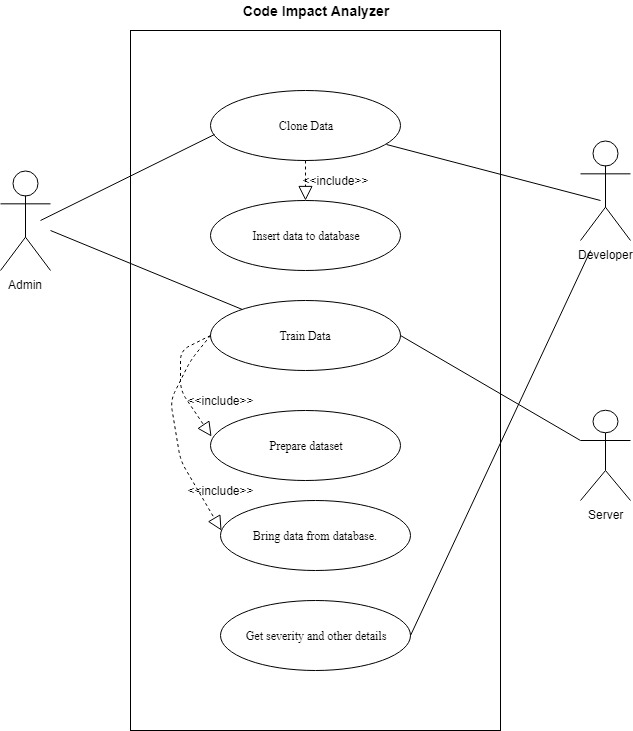
\includegraphics[width=\textwidth]{use case.jpg}
\begin{figure}[h]
    \caption{Use Case Diagram}
    \label{fig:Use Case Diagram}
\end{figure}

\subsection{Class Diagram}
\vspace*{1\baselineskip}
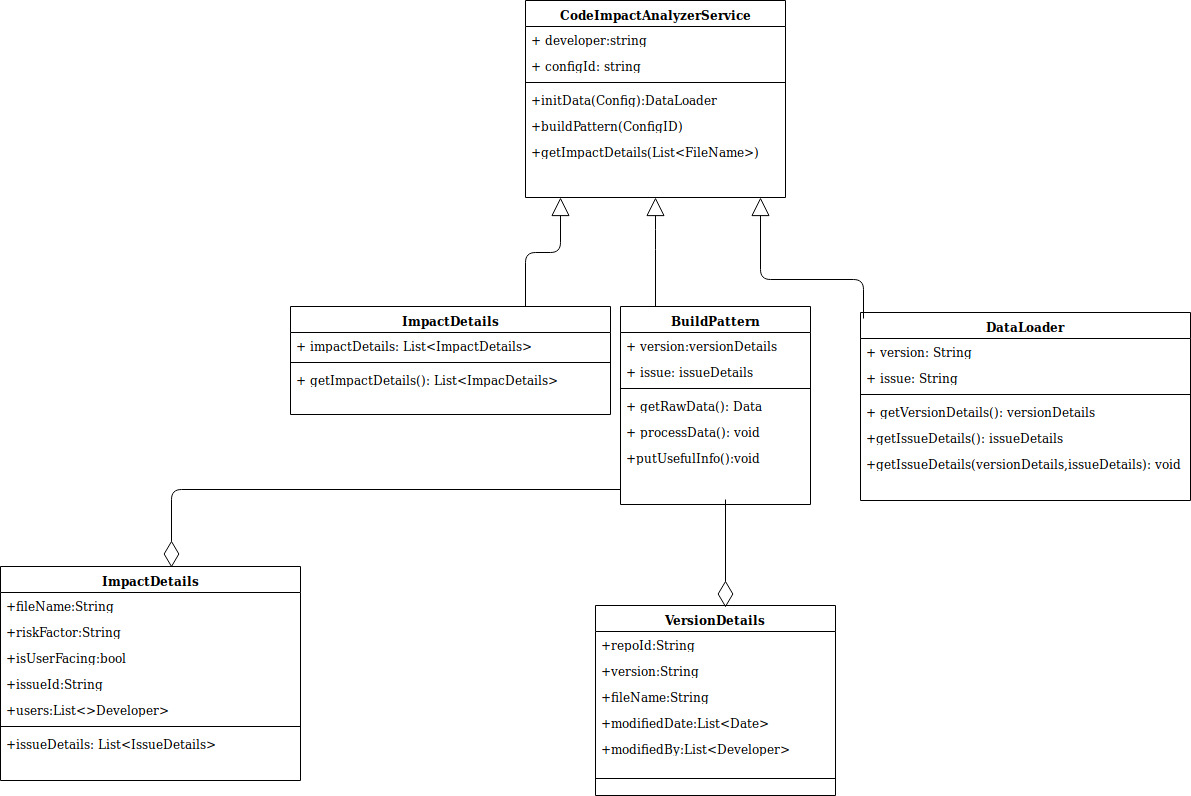
\includegraphics[width=\textwidth]{class.png}
\begin{figure}[h]
    \caption{Class Diagram}
    \label{fig:Class Diagram}
\end{figure}


\subsection{System Flow Diagram}
\vspace*{1\baselineskip}
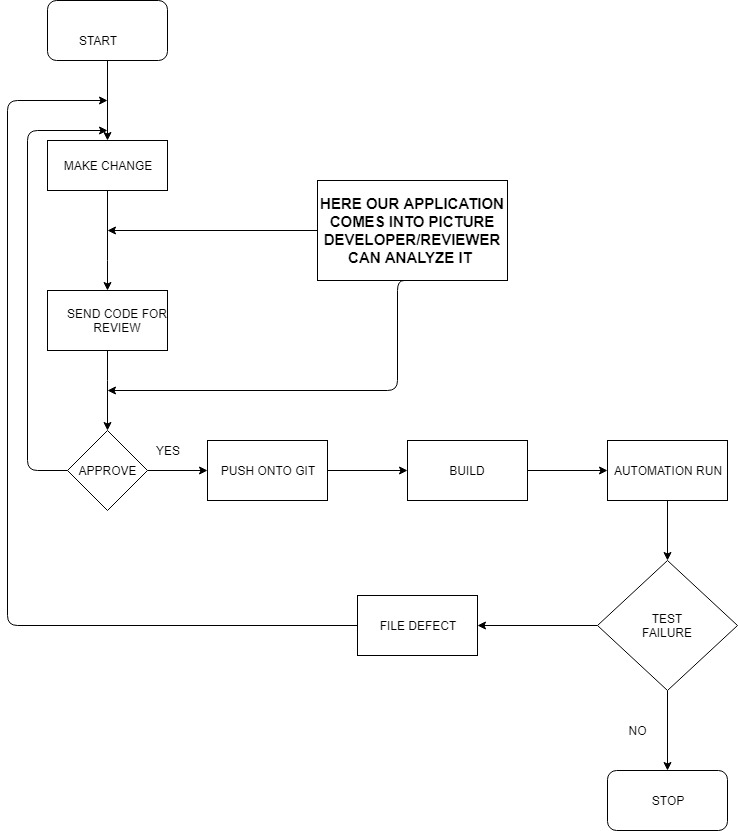
\includegraphics[width=\textwidth]{flow.png}
\begin{figure}[h]
    \caption{System Flow Diagram}
    \label{fig:System Flow Diagram}
\end{figure}

\subsection{Activity Diagram}
\begin{figure}[h]
\begin{Center}
    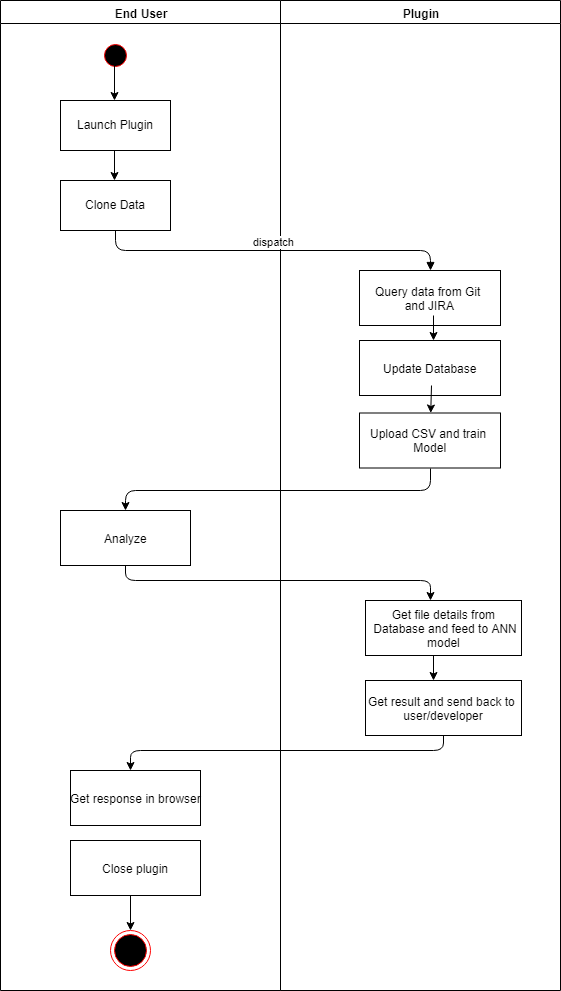
\includegraphics[width=4.4in,height=7in]{Activity.png}
    \caption{Activity Diagram}
    \label{fig:Activity Diagram}
    \end{Center}
\end{figure}
\newpage

\chapter{Project Plan}

\section{Project Estimate}

\subsection*{5.1.1\hspace*{10pt}Reconciled Estimates}
\addcontentsline{toc}{subsection}{5.1.1\hspace*{10pt}Reconciled Estimates}


\subsubsection*{5.1.1.1\hspace*{10pt}Cost Estimate}
\addcontentsline{toc}{subsubsection}{5.1.1.1\hspace*{10pt}Cost Estimate}
\setlength{\parskip}{0.0pt}
\begin{itemize}
	\item Dataset available from BMC Software.\par

	\item Required softwares are provided by BMC software.\par

	\item Required hardwares are provided by BMC software.
\end{itemize}\par


\subsubsection*{5.1.1.2\hspace*{10pt}Time Estimates}
\addcontentsline{toc}{subsubsection}{5.1.1.2\hspace*{10pt}Time Estimates}
\begin{itemize}
	\item Time estimation of project is around 6 to 8 months.
\end{itemize}\par


\section{Project Resources}

\subsection{Human Resources}


\par Human Resources: Project group members.


\begin {table*}[!htpb]
\renewcommand{\arraystretch}{1.3}
    \begin{tabular}{ l l }
        \textbf{Internal Guide:} & Prof. K. C. Waghmare \\
        \textbf{Group Members:} & Ameya Babhulgaonkar\\
        & Chaitnya Joshi\\
        & Prashant Bhivsane\\
        & Rohit Doshi\\
    \end{tabular}
\end {table*}
\newpage
\subsection{Software Resources}
\begin{enumerate}
    \item Eclipse\par
    \item Python(3.7)\par
    \item Jupyter Notebook\par
    \item JRE \par
\end{enumerate}
\subsection{Hardware Resources}
\begin{enumerate}
    \item 2.9 GHz CPU\par
    \item 8GB RAM\par
\end{enumerate}


\section{Risk Management}

\subsection{Risk Identification and Analysis}

\begin{justify}
For risks identification, review of scope document, requirements specifications and schedule is done. Answers to questionnaire revealed some risks. Please refer \setlength{\parskip}{0.0pt}
\begin{enumerate}
	\item Our project is sponsored by BMC software. The software and customer managers from the company are formally committed to support our project. 
\end{enumerate}
\end{justify}\par

	\item Communication between end user and developers is done in order to build the project.\par

	\item  All hardware and software requirements are stable and completely understood by the entire developer team as well as our end user.\par

	\item End-users expectations are taken into consideration while developing the project. \par

	\item The software team have all the required skills for carrying out the project with given specification.\par

	\item The team contains four people. They are adequate enough to do the job.\par


\subsection{Overview of Risk Mitigation, Monitoring, Management}

\begingroup
\setlength{\tabcolsep}{5pt} % Default value: 6pt
\renewcommand{\arraystretch}{1.5} % Default value: 1


\begin{table}[H]
 			\centering
\begin{tabular}{p{1.0in}p{1.35in}p{0.7in}}
\hline
%row no:1
\multicolumn{1}{|p{1.0in}}{\Centering Impact} & 
\multicolumn{1}{|p{1.18in}}{\Centering Value} & 
\multicolumn{1}{|p{3in}|}{\Centering Description}\\
\hline
%row no:2
\multicolumn{1}{|p{1.0in}}{\Centering Very high} & 
\multicolumn{1}{|p{1.18in}}{\Centering $>$ 10$\%$ } & 
\multicolumn{1}{|p{3in}|}{Schedule impact or Unacceptable quality} \\
\hline
%row no:3
\multicolumn{1}{|p{1.0in}}{\Centering High} & 
\multicolumn{1}{|p{1.18in}}{\Centering 5 $-$  10$\%$ } & 
\multicolumn{1}{|p{3in}|}{Schedule impact or Some parts of the project have low quality} \\
\hline
%row no:4
\multicolumn{1}{|p{1.0in}}{\Centering Medium} & 
\multicolumn{1}{|p{1.18in}}{\Centering $<$ 5$\%$ } & 
\multicolumn{1}{|p{3.00in}|}{Schedule impact or Barely noticeable degradation in quality Low Impact on schedule or Quality can be incorporated} \\
\hline

\end{tabular}\caption{Risk Impact Definitions }
\label{tab:Risk Impact Definitions }

 \end{table}
\endgroup






\begingroup
\setlength{\tabcolsep}{5pt} % Default value: 6pt
\renewcommand{\arraystretch}{1.5} % Default value: 1

\begin{table}[H]
 			\centering
\begin{tabular}{p{1.31in}p{3.71in}}
\hline
%row no:1
\multicolumn{1}{|p{1.31in}}{Risk ID} & 
\multicolumn{1}{|p{3.71in}|}{1} \\
\hline
%row no:2
\multicolumn{1}{|p{1.31in}}{Risk Description} & 
\multicolumn{1}{|p{3.71in}|}{JIRA Connection times out} \\
\hline
%row no:3
\multicolumn{1}{|p{1.31in}}{Category} & 
\multicolumn{1}{|p{3.71in}|}{Runtime Environment.} \\
\hline
%row no:4
\multicolumn{1}{|p{1.31in}}{Source} & 
\multicolumn{1}{|p{3.71in}|}{Data fetching jar} \\
\hline
%row no:5
\multicolumn{1}{|p{1.31in}}{Probability} & 
\multicolumn{1}{|p{3.71in}|}{Medium} \\
\hline
%row no:6
\multicolumn{1}{|p{1.31in}}{Impact} & 
\multicolumn{1}{|p{3.71in}|}{High} \\
\hline
%row no:7
\multicolumn{1}{|p{1.31in}}{Response} & 
\multicolumn{1}{|p{3.71in}|}{Mitigate} \\
\hline
%row no:8
\multicolumn{1}{|p{1.31in}}{Strategy} & 
\multicolumn{1}{|p{3.71in}|}{Always making sure that JIRA is accessible all the time.} \\
\hline
%row no:9
\multicolumn{1}{|p{1.31in}}{Risk Status} & 
\multicolumn{1}{|p{3.71in}|}{Occurred} \\
\hline

\end{tabular}
\caption{Risk Identification Table 1 }
\label{tab:Risk Identification Table 1 }

 \end{table}
\endgroup 
 
 \begingroup
\setlength{\tabcolsep}{5pt} % Default value: 6pt
\renewcommand{\arraystretch}{1.5} % Default value: 1
 
 \begin{table}[H]
 			\centering
\begin{tabular}{p{1.31in}p{3.71in}}
\begin{table}[H]
 			\centering
\begin{tabular}{p{1.31in}p{3.71in}}
\hline
%row no:1
\multicolumn{1}{|p{1.31in}}{Risk ID} & 
\multicolumn{1}{|p{3.71in}|}{2} \\
\hline
%row no:2
\multicolumn{1}{|p{1.31in}}{Risk Description} & 
\multicolumn{1}{|p{3.71in}|}{Loss of connectivity with AR system server} \\
\hline
%row no:3
\multicolumn{1}{|p{1.31in}}{Category} & 
\multicolumn{1}{|p{3.71in}|}{Deployment Environment} \\
\hline
%row no:4
\multicolumn{1}{|p{1.31in}}{Source} & 
\multicolumn{1}{|p{3.71in}|}{Server} \\
\hline
%row no:5
\multicolumn{1}{|p{1.31in}}{Probability} & 
\multicolumn{1}{|p{3.71in}|}{Low} \\
\hline
%row no:6
\multicolumn{1}{|p{1.31in}}{Impact} & 
\multicolumn{1}{|p{3.71in}|}{High} \\
\hline
%row no:7
\multicolumn{1}{|p{1.31in}}{Response} & 
\multicolumn{1}{|p{3.71in}|}{Mitigate} \\
\hline
%row no:8
\multicolumn{1}{|p{1.31in}}{Strategy} & 
\multicolumn{1}{|p{3.71in}|}{Making sure no other server is accessing the \break port used by flask server} \\
\hline
%row no:9
\multicolumn{1}{|p{1.31in}}{Risk Status} & 
\multicolumn{1}{|p{3.71in}|}{Identified} \\
\hline

\end{tabular}
\caption{Risk Identification Table 2 }
\label{tab:Risk Identification Table 2 }


 \end{table}




\end{tabular}
 \end{table}


 

\endgroup


\section{Project Schedule}

\subsection{Project Task Set}
Major Tasks in the Project stages are:\par

\setlength{\parskip}{0.0pt}
	\item Task 1: Collection of data from Git and JIRA\par

	\item Task 2: Mapping Git data with JIRA data.\par

	\item Task 3: Preparing labelled dataset using K-means clustering algorithm.\par

	\item Task 4: Training model and deploying it.\par

	\item Task 5: Developing eclipse plug-in.\par

\setlength{\parskip}{9.96pt}
	\item Task 6: Developing UI.\par
\subsection*{5.3.2\hspace*{10pt}Task network}
\addcontentsline{toc}{subsection}{5.3.2\hspace*{10pt}Task network}
\begin{Center}


%%%%%%%%%%%%%%%%%%%% Figure/Image No: 6 starts here %%%%%%%%%%%%%%%%%%%%

\begin{figure}[H]
	\begin{Center}
		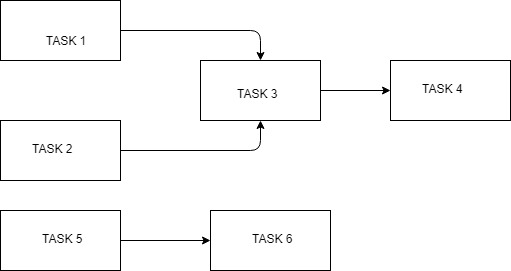
\includegraphics[width=5.32in,height=2.82in]{Tasknw.jpg}}}
		\caption{Task network}
		\label{fig:Task_network}
	\end{Center}
\end{figure}


\end{Center}\par
\subsection*{5.3.3\hspace*{10pt}Timeline Chart}
\addcontentsline{toc}{subsection}{5.3.3\hspace*{10pt}Timeline Chart}
\begin{Center}


%%%%%%%%%%%%%%%%%%%% Figure/Image No: 7 starts here %%%%%%%%%%%%%%%%%%%%

\begin{figure}[H]
	\begin{Center}
		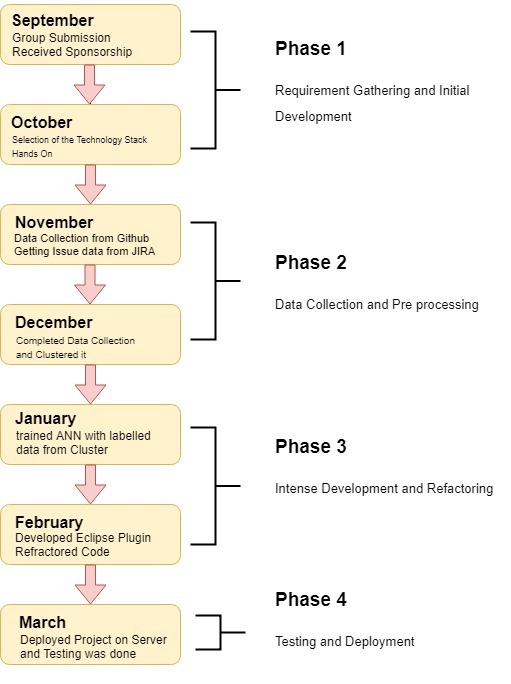
\includegraphics[width=5.43in,height=5.27in]{gc.jpg}
		\caption{Timeline Chart}
		\label{fig:Timeline_Chart}
	\end{Center}
\end{figure}

\end{Center}\par
\newpage
\section*{5.4\hspace*{10pt}Team Organization}
\addcontentsline{toc}{section}{5.4\hspace*{10pt}Team Organization}
\setlength{\parskip}{0.0pt}
\begin{itemize}
	\item Google Drive: For sharing data and files among team members.\par

	\item BMC server: For backup and data storage.\par

	\item Skype for Business: Team members communicate as and when necessary.\par

	\item BMC conference room/ College campus: Weekly meeting for discussing progress with mentor.
\end{itemize}\par
\setlength{\parskip}{9.96pt}
\subsection*{5.4.1\hspace*{10pt}Team structure}
\addcontentsline{toc}{subsection}{5.4.1\hspace*{10pt}Team structure}
\tab  Guides: To monitor the progress of the project.\par

\tab Mentor: To help in planning and assigning the tasks. To review the work done and provide suggestions and improvements required.\par

Team member 1: Front-end Development( HTML, CSS etc.) and data collection and database.\par

Team member 2: Plugin Development.\par

Team member 3: Back-end(REST, Java)\par

Team member 4: Back-end Development(ANN model development and deployment over server)\par

\subsection*{5.4.2\hspace*{10pt}Management reporting and communication}
\addcontentsline{toc}{subsection}{5.4.2\hspace*{10pt}Management reporting and communication}
Timetable was put up and sufficient time was provided for:\par

\setlength{\parskip}{0.0pt}
\begin{enumerate}
	\item Deciding the domain.\par

	\item Designing the final problem statement. \par

	\item Choosing a base paper and all support technical papers.\par

	\item Submitting group details and problem statement.\par

	\item Submission of abstract of the project.\par

	\item Submission of Synopsis and Mathematical Model.\par

	\item Literature survey.\par

	\item Review 1 with the guide and experts.\par

	\item Implementation of some part of the project.\par

	\item Review 2 with guide and experts.\par

	\item Submission of project lab assignments including UML diagrams.\par

	\item Updating project workbook regularly. \par

	\item Submission of preliminary project report.\par

	\item Review 3 with the guide and experts.\par

	\item Implementation of the project.\par

	\item Review 4 with the guide and experts.\par

	\item Submission of Project Report
\end{enumerate}\par



 %%%%%%%%%%%%  Starting New Page here %%%%%%%%%%%%%%

\newpage


\pagebreak\par

\chapter{PROJECT IMPLEMENTATION}


\vspace{\baselineskip}



 
\section{Overview of Project Modules}

\subsection{Introduction}


\begin{justify}
\tab For\ developing plugin, we used Eclipse Plugin Development Environment. REST calls are written in python language. REST calls  to the BMC server were given using Java. All the resources are deployed over Flask server. 
\end{justify}\par

\begin{justify}
\tab For gathering dataset, Git repositories were cloned through JGit API and corresponding JIRA entries were fetched using Atlassian JIRA API. Data is stored in PostGRES database. 
\end{justify}\par

\begin{justify}
\tab Webpage opened in browser is designed in HTML, CSS, Bootstrap Framework and Jinja languages.
\end{justify}\par


\section{Tools and Technologies Used}


\begin{enumerate}
	\item HTML: HyperText Markup Language is the standard language used to create web pages and web applications. HTML describes structure of web pages using HTML elements which are building blocks of web pages.\par

	\item REST API: RESTful API (Representational State Transfer Application Program Interface) is an architectural style to communicate in web services development by using HTTP requests to GET, PUT, POST and DELETE data. These APIs are written in Python language.\par

	\item Python: Python is an interpreted high-level programming language used for general-purpose programming. Watson Conversation provides python APIs to integrate with the dialog tools.\par

	\item BMC Server Machines: These are the servers which are internal to BMC, Pune and are used for deploying a flask server.\par

	\item Flask: Flask is a micro web framework written in Python. All the REST resources were deployed over this server. Flask server runs over BMC Server machines. It contains development server and debugger and also used Jinja2 templating.\par

	\item Jinja2:\ Jinja2 is a modern day templating language for Python development.  It is used to create HTML, XML or other markup formats that are returned to user via an HTTP request. \par

	\item PostGRES: We have used PostGRES database for storing all the records about the file. PostGRES is a ‘open source object relational database management system’. It can handle range of load from small single-user applications to multi-user Internet applications wherein concurrent requests are made to database. \par

	\item Eclipse Plugin Development Environment: Eclipse Plugin Development Environment (PDE) provides a efficient tools for creating, developing, deploying, testing and maintaining Eclipse plug-ins. It also provides comprehensive OSGi tooling, which makes it an ideal environment for component programming.
\end{enumerate}\par


\section{Algorithm Details}

The different modules in the project are as follows:\par

\setlength{\parskip}{0.0pt}
\begin{enumerate}
	\item Data\ Collection module:This module deals with cloning of data from BMC GitHub repository and JIRA. This module also deals with mapping the issue in Git with the issue entries in JIRA.  It also establishes connection with the Git repository and JIRA. Data gathered is in the form of .csv file.\par

	\item Database\ module: In this module, data gathered from different branches of  same project is inserted into a PostGRES database. Also a file containing entries for all branches of a project is generated. Attributes of table are number of authors, number of committers, number of revisions, number of lines changed, number of issue, severity of issue raised, kickback count, regression count, problem area etc.\par

	\item Upload data and train module: This module uploads csv file generated over a local file systems to server through a java code. After uploading this module classifies the data in this file into three severity classes namely low, medium and high using K-means algorithm and generates a csv with labelled classes. The labelled file is then used for training ANN model and trained model is then stored over a server.\par

	\item Analyze file module: This module includes a REST call to a service which fetches required details from database against a name of file and passes them to a trained model which is specific to that branch. It gives back result in the form of severity class to end user which opens up a browser on end user’s machine.\par

	\item Delta module: When user tries to clone a repository again, this module helps in bringing only those records which were added after last clone of repository instead of brining entire repository. Code is written in Java. Thus is also updates the necessary entries in database.
\end{enumerate}\par

\subsection{Algorithm 1/ Pseudocode}

\begin{enumerate}
	\item User gives/provides project name, branch name, URL of Git repository as input to fetch module.\par

	\item Based on this input, the git repositories and JIRA details are fetched from github.bmc.com and jira.bmc.com.\par

	\item All the details fetched in the previous step are written to a csv file.\par

	\item Data in csv file is inserted into a database and a merged csv is created which includes data from all the branches of given project.\par

	\item Merged csv is uploaded to a server and is given to ANN algorithm for training.\par

	\item Model is saved with $<$project\_name$>$.h5.\par

	\item When user enters a file name



\begin{justify}
7.1 Details associated with file name are fetched from database.
\end{justify}\par




\begin{justify}
7.2 Number of issues, number of revisions and number of lines changed \tab are given to built model and class is predicted against of it.
\end{justify}\par



\begin{justify}
\item   Severity class is returned to user through REST communication. 
\end{justify}\par

\end{enumerate}\par

\subsection{Working Model of Code Impact Analyzer}

\begin{figure}[H]
	\begin{Center}
		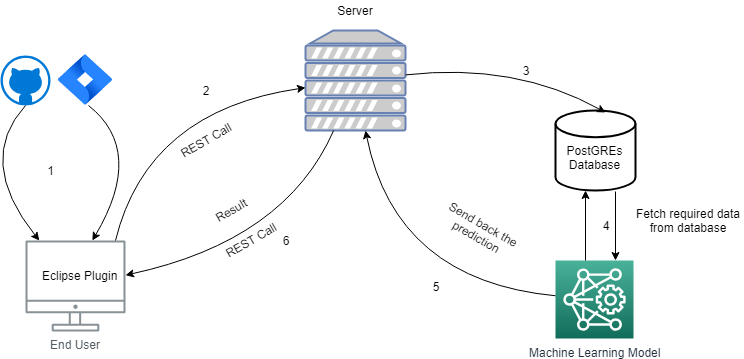
\includegraphics[width=6in,height=3.47in,scale=1.5]{Working.png}
		\caption{Working of Code Impact Analyzer}
		\label{fig:Working of Code Impact Analyzer}
	\end{Center}
\end{figure}


\newpage
\chapter{Software Testing}

\section{Goals of Testing}
\begin{itemize}
    \item To determine the usablity of application\par
    \item As the plug-in is going to be used in the organization, we have to make sure that no test case remains unhandled.\par
    
    \item As there is involvement of BMC Server, we have to insure that how multiple clients work concurrently.\par
\end{itemize}

\section{Test Objective}
\begin{itemize}
    \item To ensure robustness of application.
    \item To make sure about applicability of software built.
    \item To ensure architectural stability of application.
\end{itemize}

\section{Testing Strategy}

\begin{itemize}
\item Unit Testing: There are multiple units/ components in our software. Unit testing is a type of testing used in which individual unit or group of related units are tested. It is a type of white box testing as internal mechanism of system is taken into consideration while testing. It is done to test if each unit is giving expected output for input. \par

\setlength{\parskip}{9.96pt}
	\item Integration testing: It is a phase in software testing in which the units or modules are combined and tested as a group. It is done after unit testing. Unit tested modules are aggregated and tests defined in integration test plan are applied on the aggregates.\par
\end{itemize}

\section{Test Cases \& Results}

\begingroup
\setlength{\tabcolsep}{5pt} % Default value: 6pt
\renewcommand{\arraystretch}{1.5} % Default value: 1
\begin{table}
\begin{tabular}{p{0.51in}p{1.73in}p{2.05in}p{1.19in}}
\hline
%row no:1
\multicolumn{1}{|p{0.51in}}{\Centering Sr. No.} & 
\multicolumn{1}{|p{1.73in}}{\Centering Test Case} & 
\multicolumn{1}{|p{2.05in}}{\Centering Expected output} & 
\multicolumn{1}{|p{1.19in}|}{\Centering Actual output} \\
\hline
%row no:2
\multicolumn{1}{|p{0.51in}}{\ \ \ \ \  1.} & 
\multicolumn{1}{|p{1.73in}}{\Centering Copy the plug-in to dropin folder of Eclipse} & 
\multicolumn{1}{|p{2.05in}}{\Centering Plugin should appear in the Eclipse} & 
\multicolumn{1}{|p{1.19in}|}{\Centering Plug-in appeared in the Eclipse.} \\
\hline
%row no:3
\multicolumn{1}{|p{0.51in}}{\ \ \ \ \  2.} & 
\multicolumn{1}{|p{1.73in}}{\Centering Launch Cloning module by clicking on icon.} & 
\multicolumn{1}{|p{2.05in}}{\Centering It should start cloning and folder should be created with project name.} & 
\multicolumn{1}{|p{1.19in}|}{\Centering Cloning started and folder is created with project name} \\
\hline
%row no:4
\multicolumn{1}{|p{0.51in}}{\ \ \ \ \  3. } & 
\multicolumn{1}{|p{1.73in}}{\Centering Enter invalid project name, Git URL and branch name.} & 
\multicolumn{1}{|p{2.05in}}{\Centering Cloning should not be started and error message should be popped up.} & 
\multicolumn{1}{|p{1.19in}|}{\Centering Cloning is not started and error message is shows up.} \\
\hline
%row no:5
\multicolumn{1}{|p{0.51in}}{\ \ \ \  4. } & 
\multicolumn{1}{|p{1.73in}}{\Centering Any of the field out of project name, URL or branch name is kept blank.} & 
\multicolumn{1}{|p{2.05in}}{\Centering Error message is returned} & 
\multicolumn{1}{|p{1.19in}|}{\Centering Error message shows up and doesn’t starts cloning.} \\
\hline
%row no:6
\multicolumn{1}{|p{0.51in}}{\ \ \ \  5. } & 
\multicolumn{1}{|p{1.73in}}{\Centering Database insertion} & 
\multicolumn{1}{|p{2.05in}}{\Centering Data in the csv generated for branch must be into table in database.} & 
\multicolumn{1}{|p{1.19in}|}{\Centering Data is inserted into table in database.} \\
\hline
%row no:7
\multicolumn{1}{|p{0.51in}}{\ \ \ \  6.} & 
\multicolumn{1}{|p{1.73in}}{\Centering Merged csv} & 
\multicolumn{1}{|p{2.05in}}{\Centering CSV must be produced which contains details of all the branches in the project.} & 
\multicolumn{1}{|p{1.19in}|}{\Centering Merged CSV is created.} \\
\hline
%row no:8
\multicolumn{1}{|p{0.51in}}{\ \ \ \  7.} & 
\multicolumn{1}{|p{1.73in}}{\Centering Update and train module} & 
\multicolumn{1}{|p{2.05in}}{\Centering Merged CSV should be uploaded to server with project name. Also csv with $<$project\_name$>$  WithClass.csv should be created} & 
\multicolumn{1}{|p{1.19in}|}{\Centering Merged CSV is uploaded and  \par \Centering $<$project\_name$>$\break WithClass.csv is generated.} \\
\hline



%row no:9
\multicolumn{1}{|p{0.51in}}{\ \ \  8.} & 
\multicolumn{1}{|p{1.73in}}{\Centering Creation of .h5 file} & 
\multicolumn{1}{|p{2.05in}}{\Centering After training of module, ANN should generate .h5 file which is saved with $<$project\_name$>$.h5} & 
\multicolumn{1}{|p{1.19in}|}{\Centering $<$project\_name$>$ \break .h5 is generated.} \\
\hline




%row no:10
\multicolumn{1}{|p{0.51in}}{\ \ \ \  9.} & 
\multicolumn{1}{|p{1.73in}}{\Centering Getting results} & 
\multicolumn{1}{|p{2.05in}}{\Centering Severity class is shown in web browser.} & 
\multicolumn{1}{|p{1.19in}|}{\Centering Final result is shown in browser.} \\
\hline

\end{tabular}
\caption{Test Cases}
\label{tab:Test Cases}


 \end{table}

\endgroup

\pagebreak


\newpage
\chapter{Results \& Performance Analysis}

\section{Outcome}

\begin{itemize}
    \item The end product of this project is an Eclipse Plugin which can be incorporated into any existing Eclipse IDE.\par
    \item Also this project helps BMC employees in glancing through the history of particular file and get all the required details while in development phase.
    
    
    \par
\end{itemize}

\newpage
\section{Screenshots}
\text{1. Code Impact Analyzer plugin appears in Eclipse}
\begin{figure}[H]
	\begin{Center}
		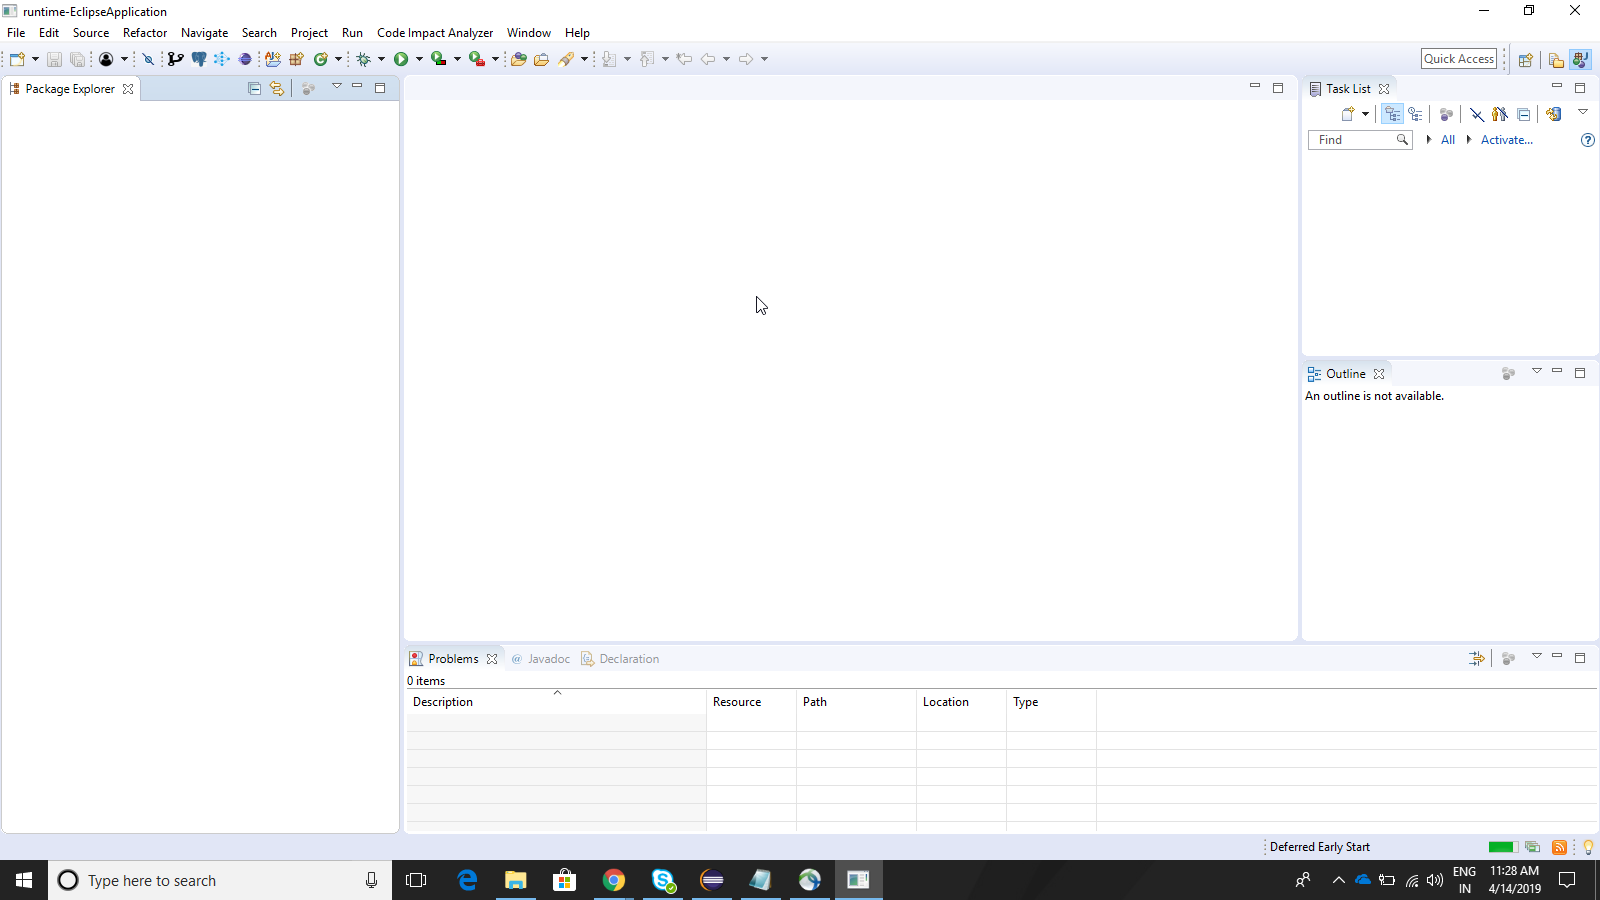
\includegraphics[width=5.75in,height=3.47in,scale=1.5]{java_kbdgDkZldh.png}
		\caption{Code Impact Analyzer plugin}
		\label{fig:Eclipse Plugin shows up in menu bar}
	\end{Center}
\end{figure}

\newpage
\begin{figure}[H]
	\begin{Center}
		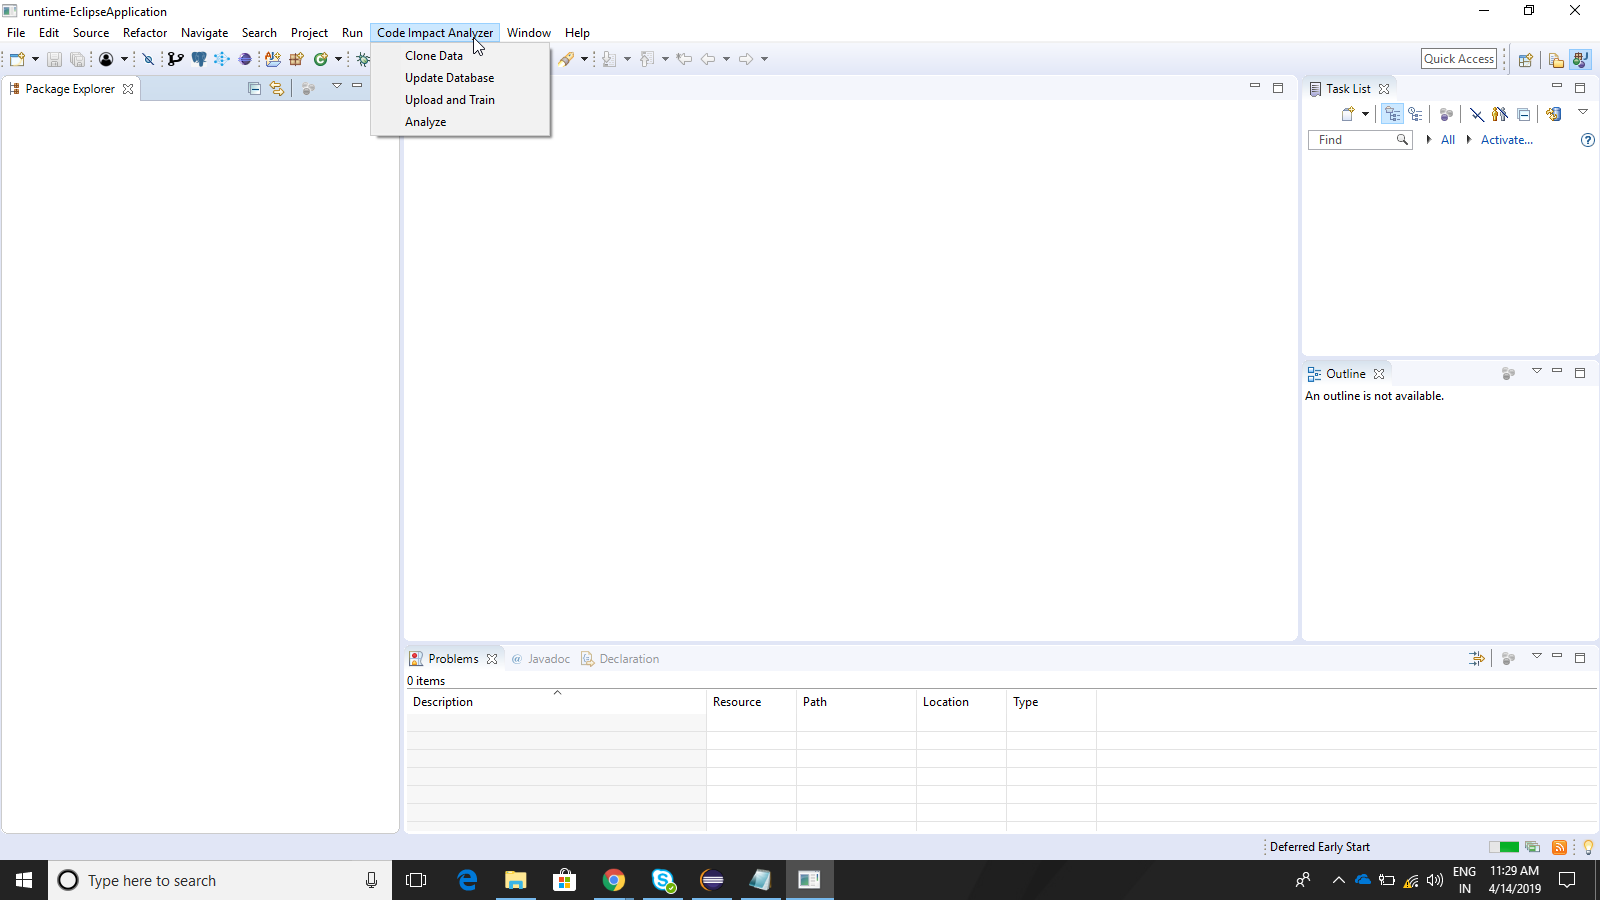
\includegraphics[width=5.75in,height=3.57in,scale=1.5]{java_nbby9ecsUh.png}
		\caption{Eclipse Plugin shows up in menu bar}
		\label{fig:Eclipse Plugin shows up in menu bar}
	\end{Center}
\end{figure}

\begin{figure}[H]
	\begin{Center}
		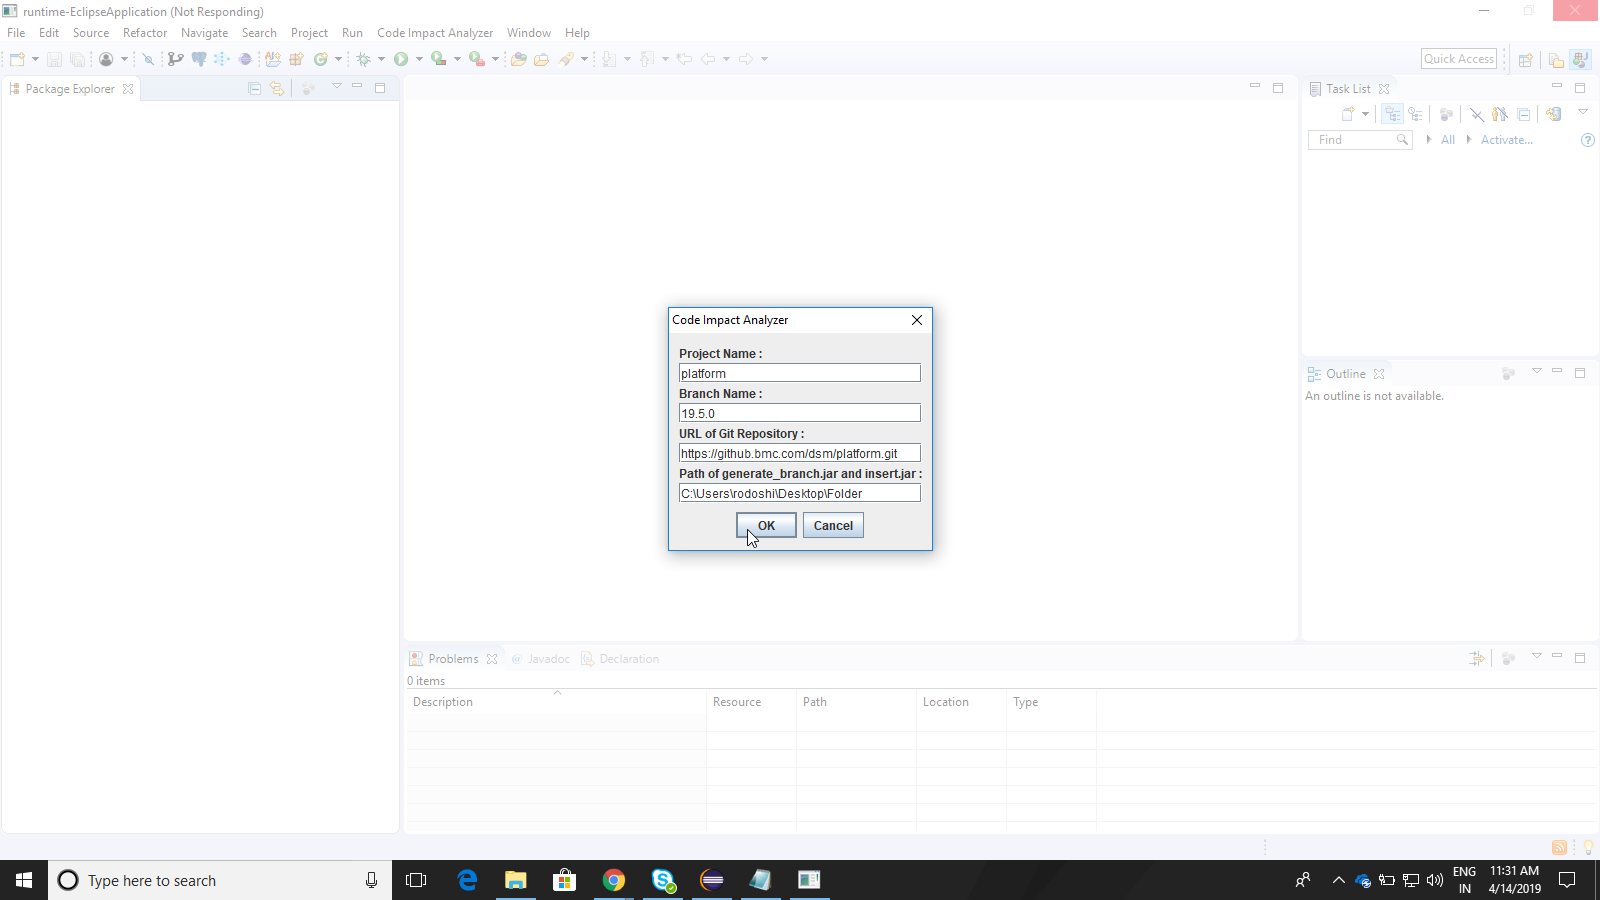
\includegraphics[width=5.75in,height=3.57in,scale=1.5]{dlRyGVSm3k.png}
		\caption{Enter required details after clicking Clone Data}
		\label{fig:Input Console}
	\end{Center}
\end{figure}

\begin{figure}[H]
	\begin{Center}
		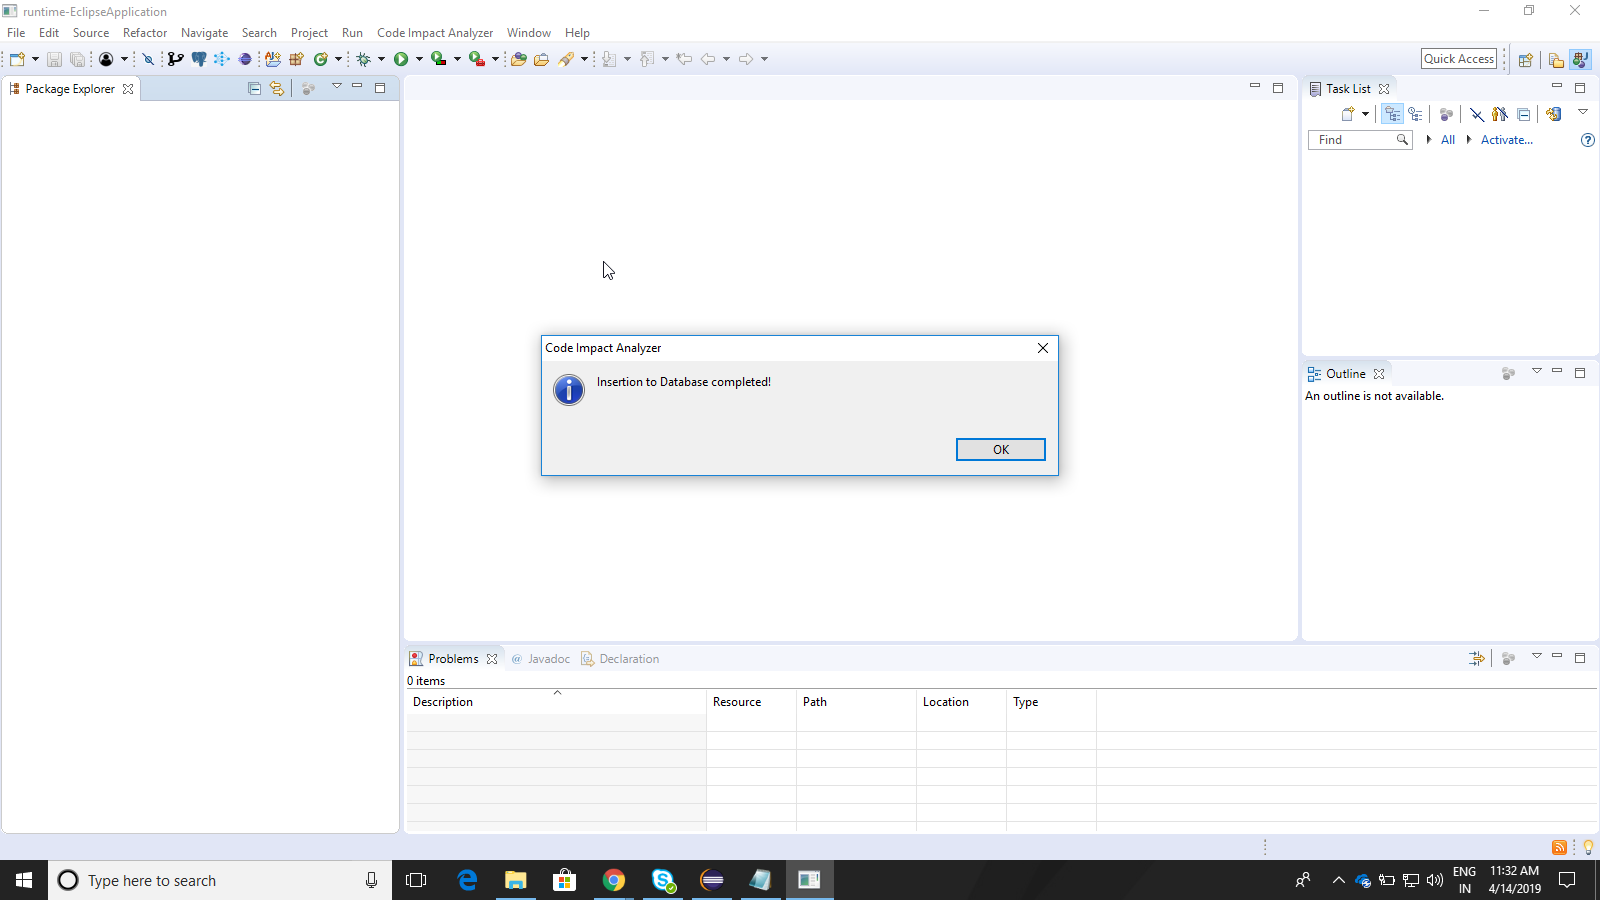
\includegraphics[width=5.75in,height=3.57in,scale=1.5]{ADxabx4JTb.png}
		\caption{Update Database Module}
		\label{fig:Update Database Module}
	\end{Center}
\end{figure}

\begin{figure}[H]
	\begin{Center}
		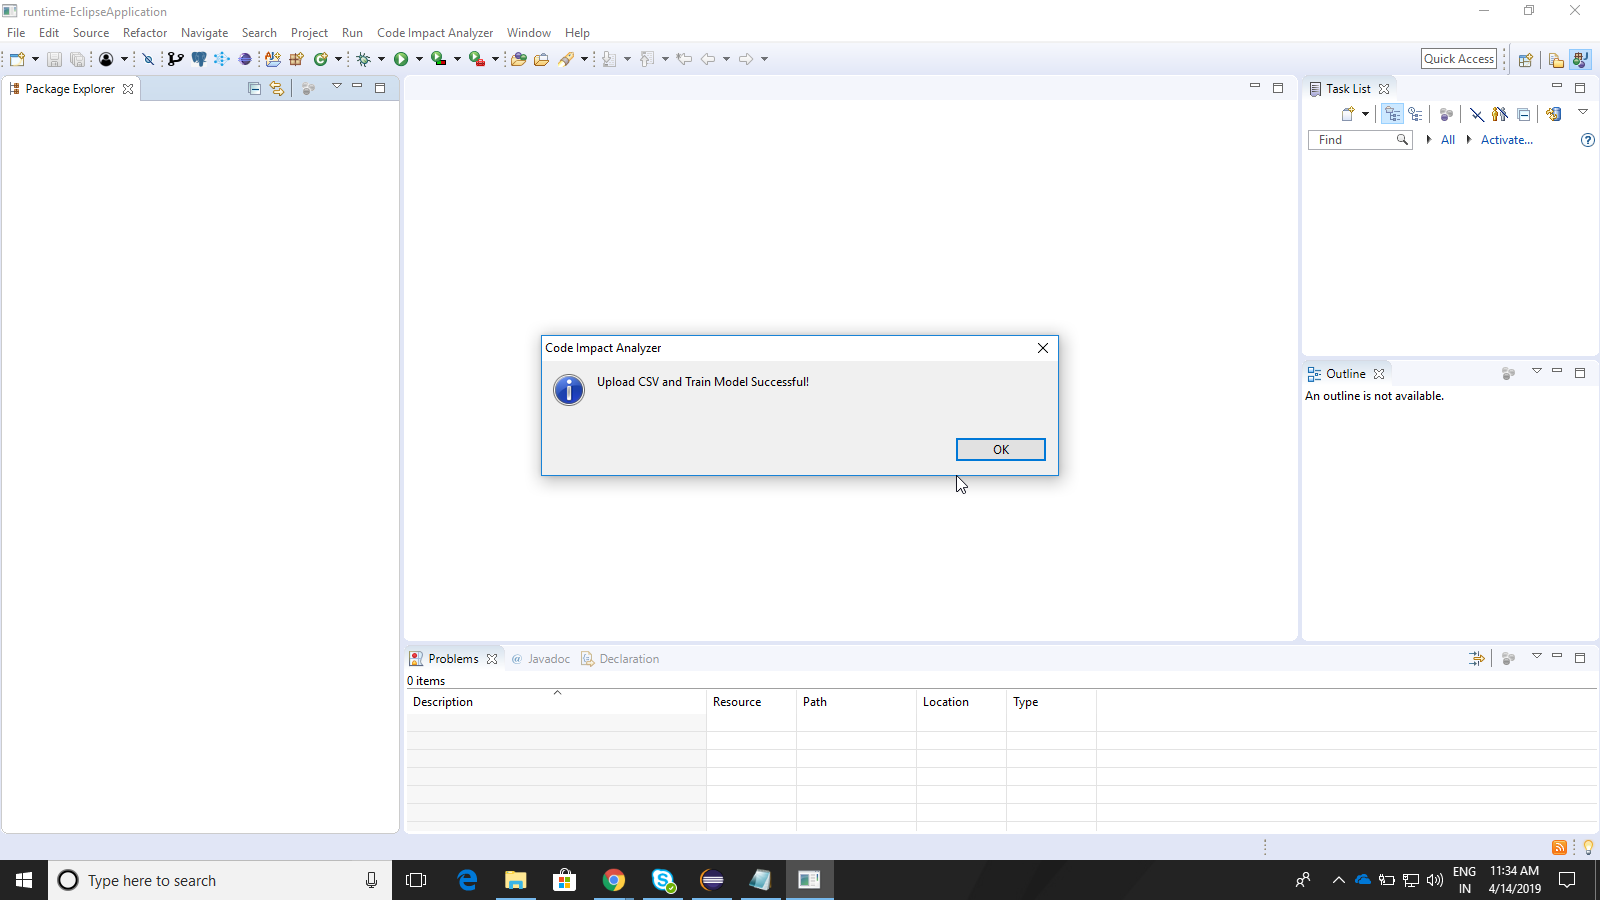
\includegraphics[width=5.75in,height=3.57in,scale=1.5]{adS89Logt1.png}
		\caption{CSV Uploading and Training  Module}
		\label{fig:CSV Uploading and Training Module}
	\end{Center}
\end{figure}


\begin{figure}[H]
	\begin{Center}
		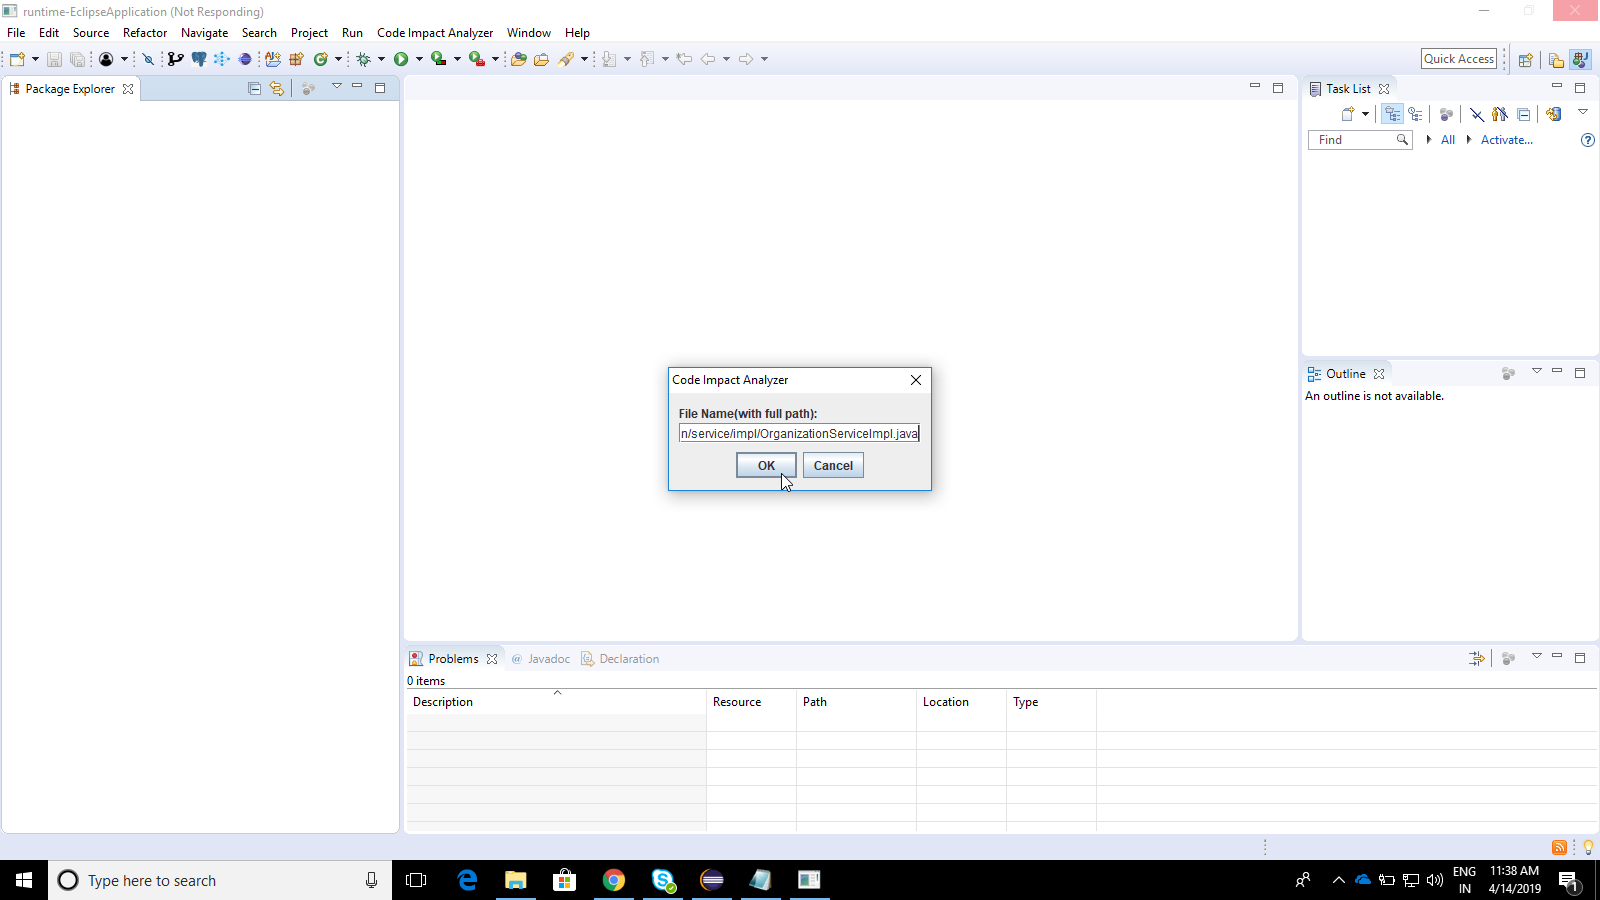
\includegraphics[width=5.75in,height=3.57in,scale=1.5]{DFasdte7Tp.png}
		\caption{Analysis  Module}
		\label{fig:Analysis Module}
	\end{Center}
\end{figure}



\begin{figure}[H]
	\begin{Center}
		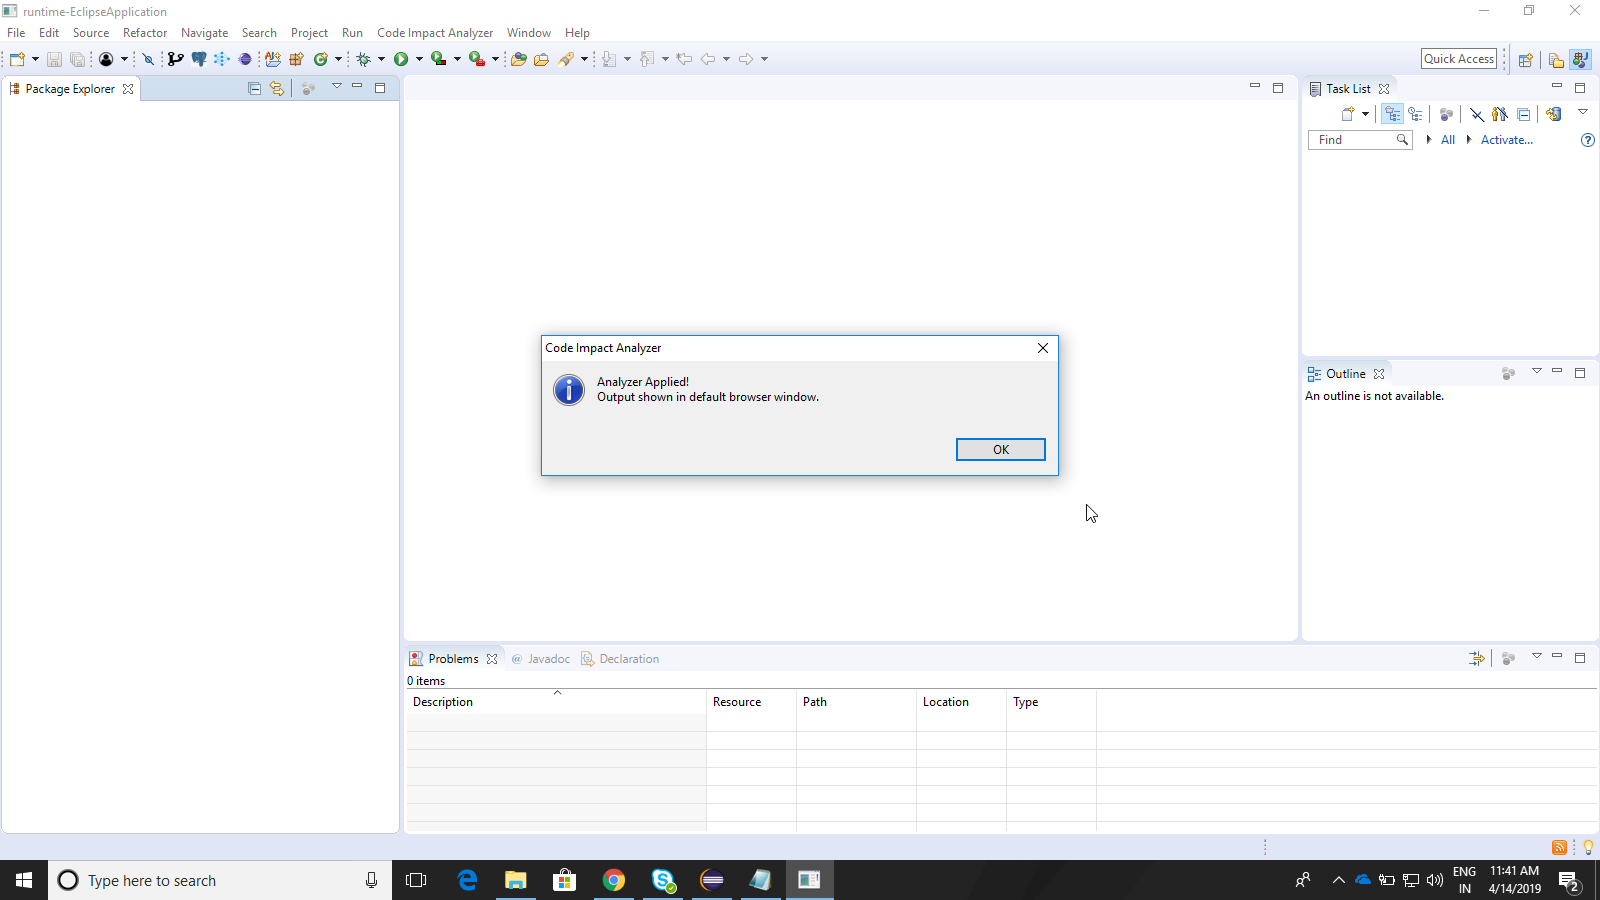
\includegraphics[width=5.75in,height=3.57in,scale=1.5]{RxAV7mor4S.png}
		\caption{Result}
		\label{fig:Result}
	\end{Center}
\end{figure}

\begin{figure}[H]
	\begin{Center}
		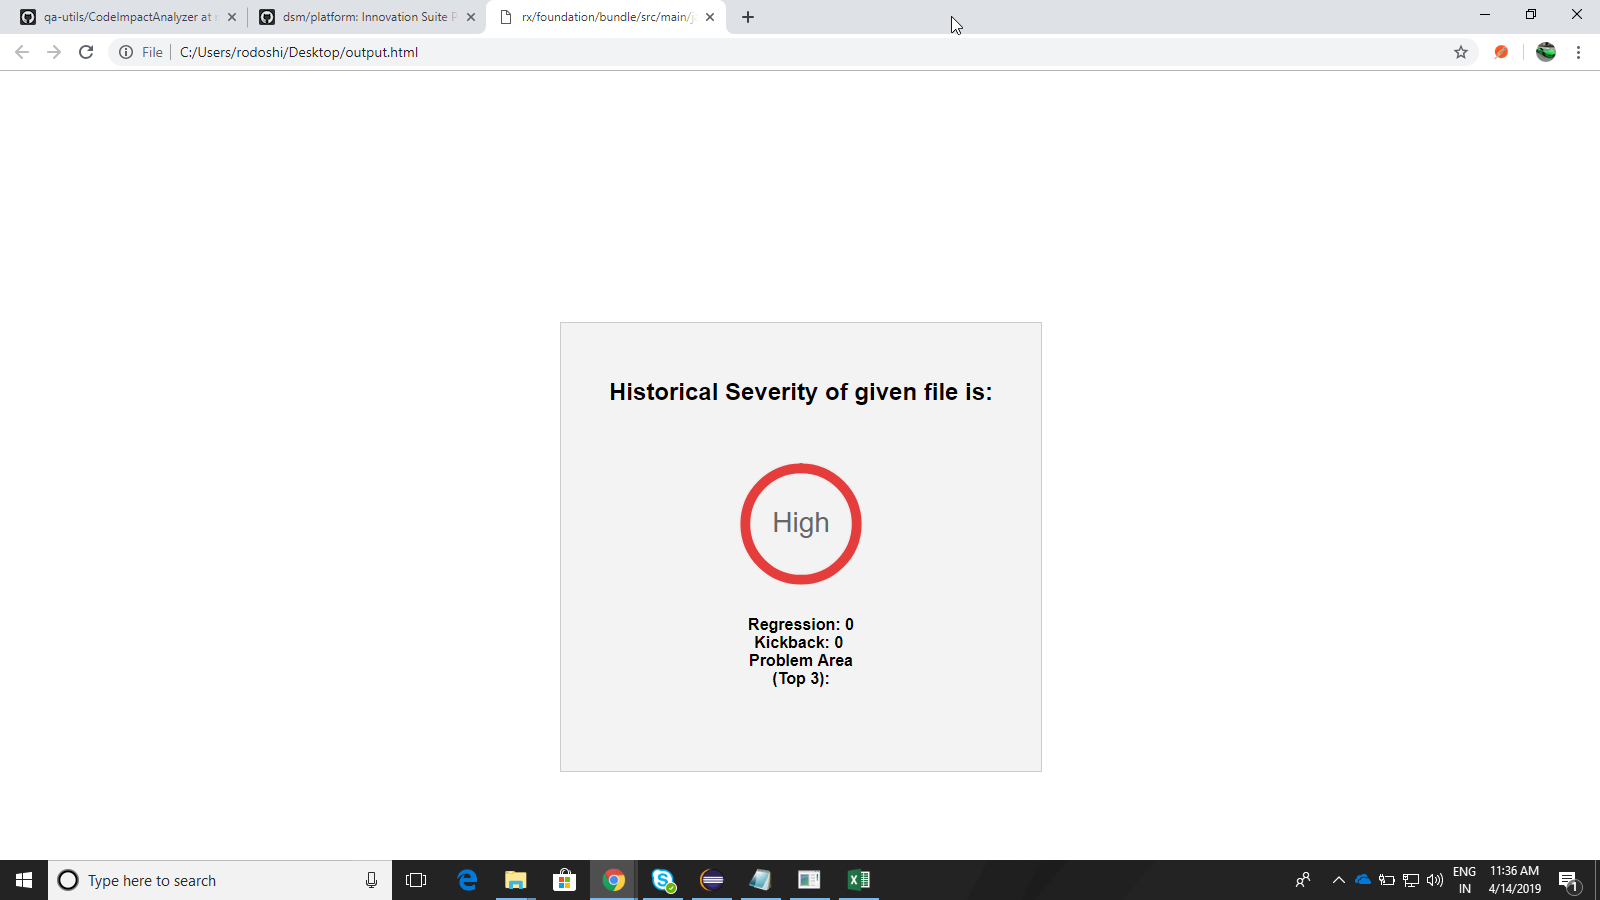
\includegraphics[width=5.75in,height=3.57in,scale=1.5]{chrome_sbdKh2cylo.png}
		\caption{Severity Class shown in browser Window}
		\label{fig:Output}
	\end{Center}
\end{figure}


\newpage
\chapter{Deployment and Maintenance}

\section{Installation}


Admin Steps:\par

\setlength{\parskip}{0.0pt}
\begin{enumerate}
	\item Copy Code Impact Analyzer jar to drop-in folder in \break C:\textbackslash Users\textbackslash $<$username$>$ \textbackslash eclipse\textbackslash java-photon2\textbackslash eclipse. \par

	\item Copy ‘generate.jar’ and ‘insertCSV.jar’ jar to any folder. Make sure you have path of it with you.\par

	\item When you hit clone option, enter branch name, project name and URL of git repository you want to clone.\par

	\item Click ‘Insert into database’ option from menu.\par

	\item Click upload and train option from menu. (This module might require time for completion as the Machine Learning Module is trained over server).\par

	\item ‘.h5 file’, which is model of ANN is downloaded on user’s machine.\par

	\item Now our model is ready to accept any input and predict its severity class.
\end{enumerate}\par

Step for next clone of repository is same.
\\
\\


End-user’s(Developer’s) steps:\par

\setlength{\parskip}{0.0pt}
\begin{enumerate}
	\item Hit ‘Analyze’ option from menu.\par

	\item It will ask for file name of file you want to analyze.\par

\setlength{\parskip}{9.96pt}
	\item Output will be shown in browser.
\end{enumerate}\par



\chapter{Conclusion}

\section{Conclusion}


\begin{justify}
\tab We have developed a Code Impact Analyzer which aims at improving development phase of software system and simplify things for BMC employee upto many extent. This system is deployed in the form of Eclipse plug-in. This system takes name of file from user and gives him/her back a severity class of it. This system attempts to analyze past history of files across all branches of a project. Responses sent by and sent back to end user(developer) is communicated through a REST call. A flask server, which is a micro web server framework, is constantly running over server. All the REST calls are responded back from this server. 
\end{justify}\par

\begin{justify}
\tab The severity class of given file is shown to user on a webpage. The ANN model is written in python language which runs over server itself. Training is module is part of REST services. The dataset used initially for training the ANN model gave us the accuracy of 84.85$\%$  which included all the branches of one project. It had around 3,73,880 records in it. We have also done Chi-square analysis over dataset which helped us to determine the feature importance of fields of data.
\end{justify}\par

\begin{justify}
\tab An Eclipse plug-in is ‘tool-at-hand’ for developer who is handling a new file which might or might not be known to him/her. In this scenario, the developed system can make the things look easier by looking at past history of project and determining severity of file at hand. Not only severity but details like Kickback count, regression count and problem area are also returned back to end user which make him/her understand complete history of file. 
\end{justify}\par

\begin{justify}
\tab We expect that this system will help employees in BMC for developing softwares. This system will surely help company to reduce the time required for Coding Phase of SDLC.
\end{justify}\par

\newpage
\section{Future Scope}

\begin{itemize}
	\item Constructs like Functions, Interfaces of standard programming languages could be taken into consideration while doing analysis of severity class of file.\par

	\item CNN algorithm can be implemented for bringing about rise in the accuracy.\par
	\item Chatbot can be developed for functionality provided by Eclipse plugin.
	
\end{itemize}\par

\newpage
\chapter{Appendix}

\newpage
\section{Appendix A}
\subsection{Euclidean Distance}
\begin{justify}
Euclidean Distance between two points in either plane or three dimensional space is the length of segment connecting those two points.If p and q are two points having n attributes each then euclidean distance between those two points is given by
\end{justify}\par

\begin{figure}[H]
	\begin{Center}
		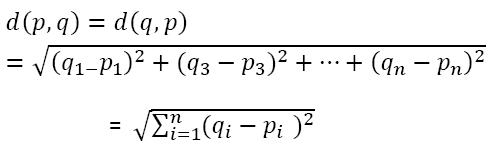
\includegraphics[width=5.15in,height=1.57in]{eiclidean.png}}
		\caption{Euclidean Distance Formula}
		\label{fig:Euclidean_Distance_Formula}
	\end{Center}
\end{figure}

\subsection{K-means Clustering Formula}


The objective of K-Means clustering is to minimize total intra-cluster variance, or, the squared error function:\par

\begin{figure}[H]
	\begin{Center}
		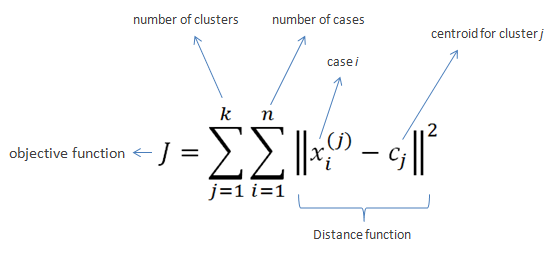
\includegraphics[width=5.15in,height=1.57in]{kmeans.png}}
		\caption{K-means equation for distance}
		\label{fig:K-means equation for distance}
	\end{Center}
\end{figure}

\newpage
\section{Appendix B}




\begin{thebibliography}{}
\bibitem{1}
L. Madeyski and M. Kawalerowicz, "Continuous Defect Prediction: The Idea and a Related Dataset," 2017 IEEE/ACM 14th International Conference on Mining Software Repositories (MSR), Buenos Aires, 2017, pp. 515-518. \newline

\bibitem{2}
G. P. Kartha, C. Anjali, R. V. Nair and S. Venkateswari, "Prediction of defect susceptibility in object Oriented Software," 2017 International Conference on Networks & Advances in Computational Technologies (NetACT), Thiruvanthapuram, 2017, pp. 467-472. \newline

\bibitem{3}
R. Karthik and N. Manikandan, "Defect association and complexity prediction by mining association and clustering rules," 2010 2nd International Conference on Computer Engineering and Technology, Chengdu, 2010, pp. V7-569-V7-573. \newline

\bibitem{4}
Y. Liu, Y. Li, J. Guo, Y. Zhou and B. Xu, "Connecting software metrics across to predict defects," 2018 IEEE 25th International Conference on Analysis, Evolution and Reengineering (SANER), Campobasso, 2018, pp. 232-243. \newline

\end{thebibliography}

\newline

\end{document}
